\documentclass[aps,prl,twocolumn,groupedaddress]{revtex4-1}
% \documentclass[aps,twocolumn,secnumarabic,balancelastpage,amsmath,amssymb,nofootinbib]{revtex4-1}
\usepackage{amsmath}
\usepackage{amssymb}
\usepackage{amsfonts}
\usepackage{color}
\usepackage{graphics}
\usepackage[pdftex]{graphicx}
\usepackage[utf8x]{inputenc}
\usepackage[colorlinks=true]{hyperref}

\newcommand{\ud}{\mathrm{d}}
\newcommand{\ue}{\mathrm{e}}
\newcommand{\ui}{\mathrm{i}}
\newcommand{\res}{\mathrm{Res}}
\newcommand{\Tr}{\mathrm{Tr}}
\newcommand{\dsum}{\displaystyle\sum}
\newcommand{\dprod}{\displaystyle\prod}
\newcommand{\dlim}{\displaystyle\lim}
\newcommand{\dint}{\displaystyle\int}
\newcommand{\fsno}[1]{{\!\not\!{#1}}}
\newcommand{\texp}[2]{\ensuremath{{#1}\times10^{#2}}}
\newcommand{\dexp}[2]{\ensuremath{{#1}\cdot10^{#2}}}
\newcommand{\eval}[2]{{\left.{#1}\right|_{#2}}}
\newcommand{\paren}[1]{{\left({#1}\right)}}
\newcommand{\lparen}[1]{{\left({#1}\right.}}
\newcommand{\rparen}[1]{{\left.{#1}\right)}}
\newcommand{\abs}[1]{{\left|{#1}\right|}}
\newcommand{\sqr}[1]{{\left[{#1}\right]}}
\newcommand{\crly}[1]{{\left\{{#1}\right\}}}
\newcommand{\angl}[1]{{\left\langle{#1}\right\rangle}}
\newcommand{\tpdiff}[4][{}]{{\paren{\frac{\partial^{#1} {#2}}{\partial {#3}{}^{#1}}}_{#4}}}
\newcommand{\tpsdiff}[4][{}]{{\paren{\frac{\partial^{#1}}{\partial {#3}{}^{#1}}{#2}}_{#4}}}
\newcommand{\pdiff}[3][{}]{{\frac{\partial^{#1} {#2}}{\partial {#3}{}^{#1}}}}
\newcommand{\diff}[3][{}]{{\frac{\ud^{#1} {#2}}{\ud {#3}{}^{#1}}}}
\newcommand{\psdiff}[3][{}]{{\frac{\partial^{#1}}{\partial {#3}{}^{#1}} {#2}}}
\newcommand{\sdiff}[3][{}]{{\frac{\ud^{#1}}{\ud {#3}{}^{#1}} {#2}}}
\newcommand{\tpddiff}[4][{}]{{\left(\dfrac{\partial^{#1} {#2}}{\partial {#3}{}^{#1}}\right)_{#4}}}
\newcommand{\tpsddiff}[4][{}]{{\paren{\dfrac{\partial^{#1}}{\partial {#3}{}^{#1}}{#2}}_{#4}}}
\newcommand{\pddiff}[3][{}]{{\dfrac{\partial^{#1} {#2}}{\partial {#3}{}^{#1}}}}
\newcommand{\ddiff}[3][{}]{{\dfrac{\ud^{#1} {#2}}{\ud {#3}{}^{#1}}}}
\newcommand{\psddiff}[3][{}]{{\frac{\partial^{#1}}{\partial{}^{#1} {#3}} {#2}}}
\newcommand{\sddiff}[3][{}]{{\frac{\ud^{#1}}{\ud {#3}{}^{#1}} {#2}}}
\newcommand{\eff}{ef\! f}
\newcommand{\fxnote}[1]{{\textbf{[#1]}}}

\newcommand{\todo}[1]{}

\ifpdf
% Ensure reproducible output
\pdfinfoomitdate=1
\pdfsuppressptexinfo=-1
\pdftrailerid{}
\hypersetup{
  pdfcreator={},
  pdfproducer={}
}
\fi

\begin{document}
\title{Coherent optical association of single molecules}
\author{Yichao Yu}
\email{yichaoyu@g.harvard.edu}
\author{Kenneth Wang}
\author{Jessie T. Zhang}
\author{Lewis Picard}
\author{William Cairncross}
\author{Kang-Kuen Ni}
\email{ni@chemistry.harvard.edu}
\affiliation{Department of Chemistry and Chemical Biology, Harvard University, Cambridge, Massachusetts, 02138, USA}
\affiliation{Department of Physics, Harvard University, Cambridge, Massachusetts, 02138, USA}
\affiliation{Harvard-MIT Center for Ultracold Atoms, Cambridge, Massachusetts, 02138, USA}

\date{\today}

\begin{abstract}
  We report coherent association of a single NaCs molecule in an optical tweezer
  through an optical Raman transition.
  By selecting a deeply bound intermediate state,
  we suppress the scattering loss during the transfer process.
  Starting from atoms in their relative motional ground state,
  we achieve optical transfer efficiency of $50 \%$ \todo{number}.
  The molecule we create have a zero-field binding energy of $770 \mathrm{MHz}$ \todo{number}
  and lifetime up to $1 \mathrm{ms}$ \todo{number}.
  We demonstrate that coherent creation of ground state single molecule is possible,
  even without Feshbach resonance or narrow optical transition.
\end{abstract}

% Coherent
% Intermediate state
% Motional state control
% Initial state preparation

\maketitle

% Introduction

Trapped neutral molecules, assembled in an array of optical tweezers,
are a promising platform to study quantum infoqrmation and quantum simulations.

\begin{figure*}
  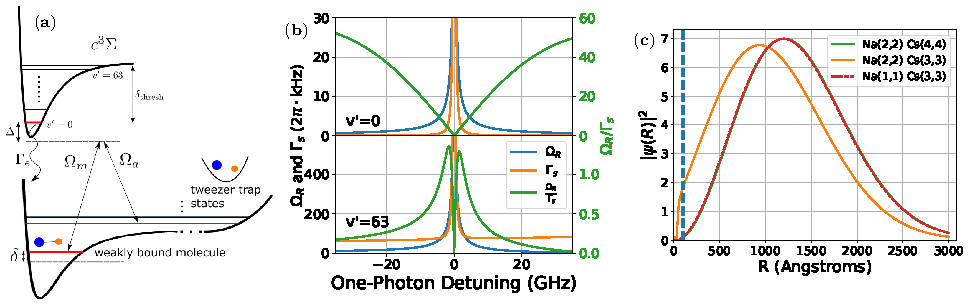
\includegraphics[height=4.5cm]{fig1.pdf}
  \caption{Optical creation of single molecule from single atoms in tweezer.
    (A) Schematics of the Raman transition. \todo{more about the states involved}
    (B) Geometry and polarization of trap and Raman beam relative to the bias magnetic field.
    \todo{Field strength, power, polarization description (pi)}
    (C) Molecule formation pulse sequence. The tweezer initially consists of only up leg power.
    This power is smoothly ramped down and the down leg power ramped up over $10\mu s$ while
    maintaining the total power of the tweezer.
    \todo{to minimize heating?}
    \label{f-setup}
  }
\end{figure*}

\begin{figure*}
  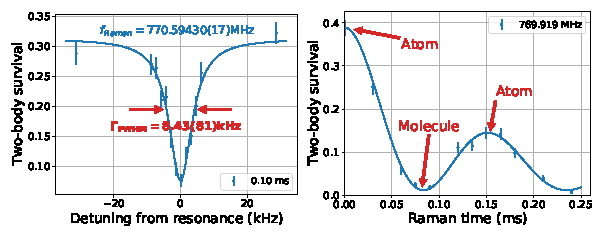
\includegraphics[height=4.5cm]{fig2.pdf}
  \caption{
    (A) Raman resonance from atomic state to molecular state, showing Fourier limited linewidth.
    \todo{states, time}
    (B) Rabi oscillation on resonance
    \label{f-raman}}
\end{figure*}

\begin{figure*}
  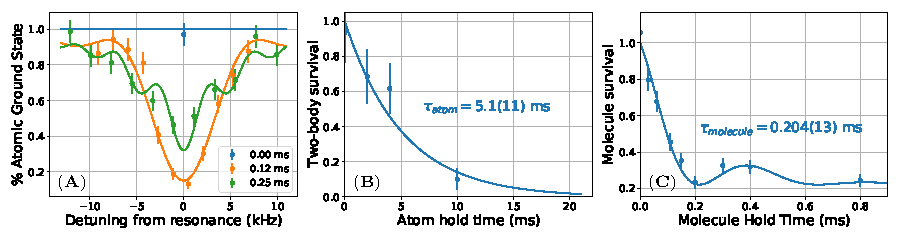
\includegraphics[height=4.5cm]{fig3.pdf}
  \caption{
    (A) Molecule lifetime in 15 mW of trap depth \todo{lifetime number}
    (B) Two-body atom lifetime in 15 mW of trap depth \todo{lifetime number,
      subtraction of single body, photoassociation rate}
    \label{f-lifetime}}
\end{figure*}

% In this Letter, we demostrate that a single ground state molecule can be formed

\bibliography{paper}
\end{document}
